% Options for packages loaded elsewhere
\PassOptionsToPackage{unicode}{hyperref}
\PassOptionsToPackage{hyphens}{url}
\PassOptionsToPackage{dvipsnames,svgnames,x11names}{xcolor}
%
\documentclass[
  article]{jss}

\usepackage{amsmath,amssymb}
\usepackage{iftex}
\ifPDFTeX
  \usepackage[T1]{fontenc}
  \usepackage[utf8]{inputenc}
  \usepackage{textcomp} % provide euro and other symbols
\else % if luatex or xetex
  \usepackage{unicode-math}
  \defaultfontfeatures{Scale=MatchLowercase}
  \defaultfontfeatures[\rmfamily]{Ligatures=TeX,Scale=1}
\fi
\usepackage{lmodern}
\ifPDFTeX\else  
    % xetex/luatex font selection
\fi
% Use upquote if available, for straight quotes in verbatim environments
\IfFileExists{upquote.sty}{\usepackage{upquote}}{}
\IfFileExists{microtype.sty}{% use microtype if available
  \usepackage[]{microtype}
  \UseMicrotypeSet[protrusion]{basicmath} % disable protrusion for tt fonts
}{}
\makeatletter
\@ifundefined{KOMAClassName}{% if non-KOMA class
  \IfFileExists{parskip.sty}{%
    \usepackage{parskip}
  }{% else
    \setlength{\parindent}{0pt}
    \setlength{\parskip}{6pt plus 2pt minus 1pt}}
}{% if KOMA class
  \KOMAoptions{parskip=half}}
\makeatother
\usepackage{xcolor}
\setlength{\emergencystretch}{3em} % prevent overfull lines
\setcounter{secnumdepth}{-\maxdimen} % remove section numbering
% Make \paragraph and \subparagraph free-standing
\ifx\paragraph\undefined\else
  \let\oldparagraph\paragraph
  \renewcommand{\paragraph}[1]{\oldparagraph{#1}\mbox{}}
\fi
\ifx\subparagraph\undefined\else
  \let\oldsubparagraph\subparagraph
  \renewcommand{\subparagraph}[1]{\oldsubparagraph{#1}\mbox{}}
\fi


\providecommand{\tightlist}{%
  \setlength{\itemsep}{0pt}\setlength{\parskip}{0pt}}\usepackage{longtable,booktabs,array}
\usepackage{calc} % for calculating minipage widths
% Correct order of tables after \paragraph or \subparagraph
\usepackage{etoolbox}
\makeatletter
\patchcmd\longtable{\par}{\if@noskipsec\mbox{}\fi\par}{}{}
\makeatother
% Allow footnotes in longtable head/foot
\IfFileExists{footnotehyper.sty}{\usepackage{footnotehyper}}{\usepackage{footnote}}
\makesavenoteenv{longtable}
\usepackage{graphicx}
\makeatletter
\def\maxwidth{\ifdim\Gin@nat@width>\linewidth\linewidth\else\Gin@nat@width\fi}
\def\maxheight{\ifdim\Gin@nat@height>\textheight\textheight\else\Gin@nat@height\fi}
\makeatother
% Scale images if necessary, so that they will not overflow the page
% margins by default, and it is still possible to overwrite the defaults
% using explicit options in \includegraphics[width, height, ...]{}
\setkeys{Gin}{width=\maxwidth,height=\maxheight,keepaspectratio}
% Set default figure placement to htbp
\makeatletter
\def\fps@figure{htbp}
\makeatother

\usepackage{orcidlink,thumbpdf,lmodern}

\newcommand{\class}[1]{`\code{#1}'}
\newcommand{\fct}[1]{\code{#1()}}
\makeatletter
\@ifpackageloaded{tcolorbox}{}{\usepackage[skins,breakable]{tcolorbox}}
\@ifpackageloaded{fontawesome5}{}{\usepackage{fontawesome5}}
\definecolor{quarto-callout-color}{HTML}{909090}
\definecolor{quarto-callout-note-color}{HTML}{0758E5}
\definecolor{quarto-callout-important-color}{HTML}{CC1914}
\definecolor{quarto-callout-warning-color}{HTML}{EB9113}
\definecolor{quarto-callout-tip-color}{HTML}{00A047}
\definecolor{quarto-callout-caution-color}{HTML}{FC5300}
\definecolor{quarto-callout-color-frame}{HTML}{acacac}
\definecolor{quarto-callout-note-color-frame}{HTML}{4582ec}
\definecolor{quarto-callout-important-color-frame}{HTML}{d9534f}
\definecolor{quarto-callout-warning-color-frame}{HTML}{f0ad4e}
\definecolor{quarto-callout-tip-color-frame}{HTML}{02b875}
\definecolor{quarto-callout-caution-color-frame}{HTML}{fd7e14}
\makeatother
\makeatletter
\makeatother
\makeatletter
\makeatother
\makeatletter
\@ifpackageloaded{caption}{}{\usepackage{caption}}
\AtBeginDocument{%
\ifdefined\contentsname
  \renewcommand*\contentsname{Table of contents}
\else
  \newcommand\contentsname{Table of contents}
\fi
\ifdefined\listfigurename
  \renewcommand*\listfigurename{List of Figures}
\else
  \newcommand\listfigurename{List of Figures}
\fi
\ifdefined\listtablename
  \renewcommand*\listtablename{List of Tables}
\else
  \newcommand\listtablename{List of Tables}
\fi
\ifdefined\figurename
  \renewcommand*\figurename{Figure}
\else
  \newcommand\figurename{Figure}
\fi
\ifdefined\tablename
  \renewcommand*\tablename{Table}
\else
  \newcommand\tablename{Table}
\fi
}
\@ifpackageloaded{float}{}{\usepackage{float}}
\floatstyle{ruled}
\@ifundefined{c@chapter}{\newfloat{codelisting}{h}{lop}}{\newfloat{codelisting}{h}{lop}[chapter]}
\floatname{codelisting}{Listing}
\newcommand*\listoflistings{\listof{codelisting}{List of Listings}}
\makeatother
\makeatletter
\@ifpackageloaded{caption}{}{\usepackage{caption}}
\@ifpackageloaded{subcaption}{}{\usepackage{subcaption}}
\makeatother
\makeatletter
\makeatother
\ifLuaTeX
  \usepackage{selnolig}  % disable illegal ligatures
\fi
\IfFileExists{bookmark.sty}{\usepackage{bookmark}}{\usepackage{hyperref}}
\IfFileExists{xurl.sty}{\usepackage{xurl}}{} % add URL line breaks if available
\urlstyle{same} % disable monospaced font for URLs
\hypersetup{
  pdftitle={Imputation of Incomplete Multilevel Data with R},
  pdfauthor={Hanne I. Oberman; Johanna Muñoz; Valentijn M.T. de Jong; Gerko Vink; Thomas P.A. Debray},
  pdfkeywords={missing data, multilevel, clustering, mice, R},
  colorlinks=true,
  linkcolor={blue},
  filecolor={Maroon},
  citecolor={Blue},
  urlcolor={Blue},
  pdfcreator={LaTeX via pandoc}}

%% -- Article metainformation (author, title, ...) -----------------------------

%% Author information
\author{Hanne I. Oberman~\orcidlink{0000-0003-3276-2141}\\Utrecht
University \And Johanna
Muñoz~\orcidlink{0000-0002-2384-5415}\\University Medical Center
Utrecht \AND Valentijn M.T. de
Jong~\orcidlink{0000-0001-9921-3468}\\University Medical Center
Utrecht \And Gerko Vink~\orcidlink{0000-0001-9767-1924}\\University
Medical Center Utrecht \AND Thomas P.A.
Debray~\orcidlink{0000-0002-1790-2719}\\University Medical Center
Utrecht}
\Plainauthor{Hanne I. Oberman, Johanna Muñoz, Valentijn M.T. de
Jong, Gerko Vink, Thomas P.A. Debray} %% comma-separated

\title{Imputation of Incomplete Multilevel Data with R}
\Plaintitle{Imputation of Incomplete Multilevel Data with
R} %% without formatting

%% an abstract and keywords
\Abstract{This tutorial illustrates the imputation of incomplete
multilevel data with the \proglang{R} packackage \pkg{mice}. Our scope
is only simple multilevel models, to show how imputation can yield less
biased estimates from incomplete clustered data. More complex models can
be accomodated, but are outside the scope of this paper. Incomplete
multilevel data requires careful consideration of the missing data
problem and analysis strategy. In this tutorial, we focus on a popular
strategy for accommodating missingness in multilevel data: replacing the
missing data with one or more plausible values, i.e.,
imputation.Imputation separates the missing data problem from the main
analysis and the completed data can be analyzed as if it has been fully
observed. This tutorial illustrates the imputation of incomplete
multilevel data with the statistical programming language R. We aim to
show how imputation can yield less biased estimates from incomplete
clustered data. We provide practical guidelines and code snippets for
different missing data situations, including non-ignorable missingness
mechanisms. For brevity, we focus on multilevel imputation using chained
equations with the R mice package and its adjacent packages.}

%% at least one keyword must be supplied
\Keywords{missing
data, multilevel, clustering, \pkg{mice}, \proglang{R}}
\Plainkeywords{missing data, multilevel, clustering, mice, R}

%% publication information
%% NOTE: Typically, this can be left commented and will be filled out by the technical editor
%% \Volume{50}
%% \Issue{9}
%% \Month{June}
%% \Year{2012}
%% \Submitdate{2012-06-04}
%% \Acceptdate{2012-06-04}
%% \setcounter{page}{1}
%% \Pages{1--xx}

%% The address of (at least) one author should be given
%% in the following format:
\Address{
Hanne I. Oberman\\
Methodology and Statistics\\
Padualaan 14\\
Utrecht The Netherlands\\
E-mail: \email{Achim.Zeileis@R-project.org}\\
URL: \url{https://www.zeileis.org/}\\
\\~
Johanna Muñoz\\
Julius Centre for Health Sciences and Primary Care\\
Universiteitsweg 100\\
Utrecht The Netherlands\\
\\~
Valentijn M.T. de Jong\\
Julius Centre for Health Sciences and Primary Care\\
Utrecht The Netherlands\\
\\~
Gerko Vink\\
Julius Centre for Health Sciences and Primary Care\\
Universiteitsweg 100\\
Utrecht The Netherlands\\
\\~
Thomas P.A. Debray\\
Julius Centre for Health Sciences and Primary Care\\
Universiteitsweg 100\\
Utrecht The Netherlands\\
\\~

}

\begin{document}
\maketitle
\hypertarget{sec-intro}{%
\section{Introduction: Clustering and incomplete data}\label{sec-intro}}

\begin{enumerate}
\def\labelenumi{\arabic{enumi}.}
\tightlist
\item
  missing data occur often in data with human subjects
\item
  missing data may be resolved, but need to be handled in accordance
  with the analysis of scientific interest
\item
  in human-subjects research, there is often clustering, which may be
  captured with multilevel modeling techniques
\item
  if the analysis of scientific interest is a multilevel model, the
  missing data handling method should accommodate the multilevel
  structure of the data
\item
  both missingness and multilevel structures require advanced
  statistical techniques
\item
  this tutorial sets out to facilitate empirical researchers in
  accommodating both multilevel structures as well as missing data.
\item
  we illustrate the use of the software by means of three case studies
  from the social and biomedical sciences.
\end{enumerate}

\hypertarget{overview-of-software}{%
\subsection{overview of software}\label{overview-of-software}}

The popular \pkg{mice} package in \proglang{R} \citet{R}\ldots{}

\hypertarget{scope}{%
\subsection{scope}\label{scope}}

\hypertarget{sec-models}{%
\section{Background}\label{sec-models}}

\hypertarget{concepts-in-multilevel-data}{%
\subsection{concepts in multilevel
data}\label{concepts-in-multilevel-data}}

\begin{tcolorbox}[enhanced jigsaw, bottomrule=.15mm, breakable, arc=.35mm, colback=white, left=2mm, toprule=.15mm, rightrule=.15mm, leftrule=.75mm, opacityback=0]

Box 1. The intraclass correlation coefficient.

\end{tcolorbox}

In \proglang{R}, multilevel models may be fitted using the package
\pkg{lme4}. For linear mixed-effects models, the function

\begin{verbatim}
lmer(formula, data, ...)
\end{verbatim}

\hypertarget{concepts-in-missing-data}{%
\subsection{concepts in missing data}\label{concepts-in-missing-data}}

The \proglang{R} package \pkg{mice} provides a framework for imputing
incomplete data on a variable-by-variable basis. The \fct{mice} function
allows users to flexibly specify how many times and under what model the
missing data should be imputed. This is reflected in the first four
function arguments

\begin{verbatim}
mice(data, m, method, predictorMatrix, ...)
\end{verbatim}

where \texttt{data} refers to the incomplete dataset, \texttt{m}
determines the number of imputations, \texttt{method} denotes the
functional form of the imputation model and \texttt{predictorMatrix}
specifies the interrelational dependencies between variables and
imputation models (i.e., the set of predictors to be used for imputing
each incomplete variable).

\begin{tcolorbox}[enhanced jigsaw, bottomrule=.15mm, breakable, arc=.35mm, colback=white, left=2mm, toprule=.15mm, rightrule=.15mm, leftrule=.75mm, opacityback=0]

Box 2. The \texttt{methods}.

\end{tcolorbox}

\begin{tcolorbox}[enhanced jigsaw, bottomrule=.15mm, breakable, arc=.35mm, colback=white, left=2mm, toprule=.15mm, rightrule=.15mm, leftrule=.75mm, opacityback=0]

Box 2. The predictor matrix.

\end{tcolorbox}

\hypertarget{sec-illustrations}{%
\section{Illustrations}\label{sec-illustrations}}

In this section, we demonstrate the workflow using three case studies.

\hypertarget{setup}{%
\subsection{Setup}\label{setup}}

\begin{verbatim}
R> library(mice)
R> library(ggmice)
\end{verbatim}

\hypertarget{popularity-data}{%
\subsection{Popularity data}\label{popularity-data}}

\begin{verbatim}
R> data("popmis", package = "mice")
\end{verbatim}

\begin{verbatim}
R> dat <- popmis[, c("school", "popular", "sex")] 
\end{verbatim}

\begin{verbatim}
R> plot_pattern(dat)
\end{verbatim}

\begin{figure}[H]

{\centering 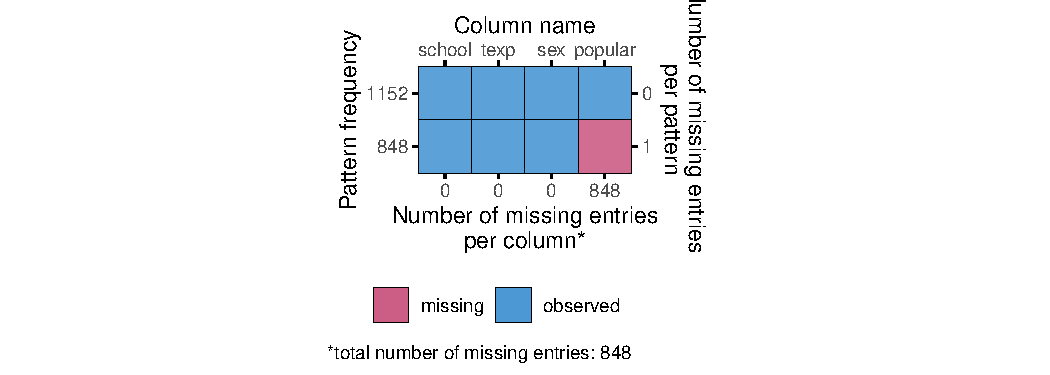
\includegraphics{manuscript_files/figure-pdf/fig-pattern-1.pdf}

}

\caption{\label{fig-pattern}Missing data pattern.}

\end{figure}

\begin{verbatim}
R> plot_corr(dat)
\end{verbatim}

\begin{figure}[H]

{\centering 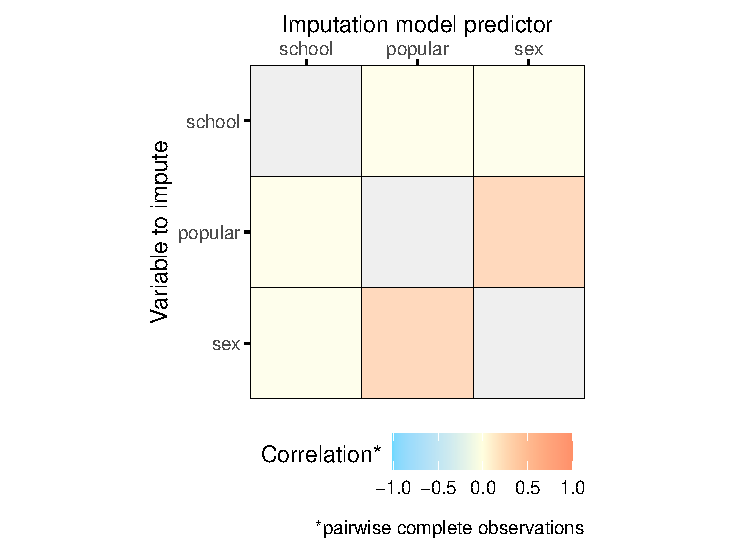
\includegraphics{manuscript_files/figure-pdf/unnamed-chunk-5-1.pdf}

}

\caption{Pair-wise correlations.}

\end{figure}

\begin{verbatim}
R> meth <- make.method(dat)
\end{verbatim}

\begin{verbatim}
R> pred <- quickpred(dat)
R> plot_pred(pred, method = meth)
\end{verbatim}

\begin{figure}[H]

{\centering 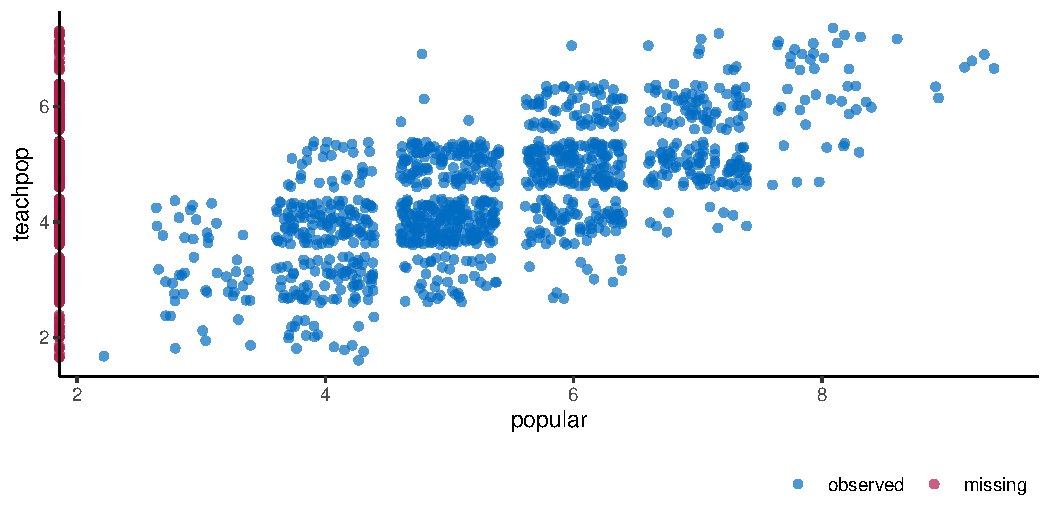
\includegraphics{manuscript_files/figure-pdf/unnamed-chunk-7-1.pdf}

}

\end{figure}

\begin{verbatim}
R> imp <- mice(
+  data = dat,
+  method = meth,
+  predictorMatrix = pred,
+  printFlag = FALSE
+)
\end{verbatim}

\begin{verbatim}
R> plot_trace(imp)
\end{verbatim}

\begin{figure}[H]

{\centering 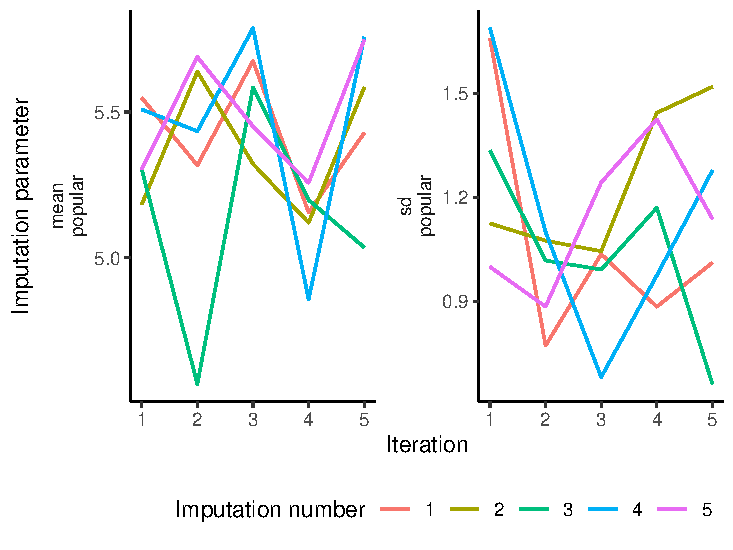
\includegraphics{manuscript_files/figure-pdf/unnamed-chunk-9-1.pdf}

}

\end{figure}

\hypertarget{sec-summary}{%
\section{Summary and discussion}\label{sec-summary}}

What is missing from this manuscript\ldots{}

\hypertarget{computational-details}{%
\section*{Computational details}\label{computational-details}}
\addcontentsline{toc}{section}{Computational details}

The results in this paper were obtained using
\proglang{R}\textasciitilde4.3.0. \proglang{R} itself and all packages
used are available from the Comprehensive \proglang{R} Archive Network
(CRAN) at {[}https://CRAN.R-project.org/{]}.

\hypertarget{acknowledgments}{%
\section*{Acknowledgments}\label{acknowledgments}}
\addcontentsline{toc}{section}{Acknowledgments}

This project has received funding from the European Union's Horizon 2020
research and innovation programme under ReCoDID grant agreement No
825746.

\hypertarget{references}{%
\section*{References}\label{references}}
\addcontentsline{toc}{section}{References}

\renewcommand{\bibsection}{}
\bibliography{bibliography.bib}

\newpage{}

\hypertarget{sec-techdetails}{%
\section*{More technical details}\label{sec-techdetails}}
\addcontentsline{toc}{section}{More technical details}

\begin{tcolorbox}[enhanced jigsaw, bottomrule=.15mm, breakable, arc=.35mm, colback=white, left=2mm, toprule=.15mm, rightrule=.15mm, leftrule=.75mm, opacityback=0]

Appendices can be included after the bibliography (with a page break).
Each section within the appendix should have a proper section title
(rather than just \emph{Appendix}).

For more technical style details, please check out JSS's style FAQ at
{[}https://www.jstatsoft.org/pages/view/style\#frequently-asked-questions{]}
which includes the following topics:

\begin{itemize}
\tightlist
\item
  Title vs.~sentence case.
\item
  Graphics formatting.
\item
  Naming conventions.
\item
  Turning JSS manuscripts into \proglang{R} package vignettes.
\item
  Trouble shooting.
\item
  Many other potentially helpful details\ldots{}
\end{itemize}

\end{tcolorbox}

\hypertarget{sec-bibtex}{%
\section*{Using BibTeX}\label{sec-bibtex}}
\addcontentsline{toc}{section}{Using BibTeX}

\begin{tcolorbox}[enhanced jigsaw, bottomrule=.15mm, breakable, arc=.35mm, colback=white, left=2mm, toprule=.15mm, rightrule=.15mm, leftrule=.75mm, opacityback=0]

References need to be provided in a \textsc{Bib}{\TeX} file
(\texttt{.bib}). All references should be made with \texttt{@cite}
syntax. This commands yield different formats of author-year citations
and allow to include additional details (e.g.,pages, chapters, \dots) in
brackets. In case you are not familiar with these commands see the JSS
style FAQ for details.

Cleaning up \textsc{Bib}{\TeX} files is a somewhat tedious task --
especially when acquiring the entries automatically from mixed online
sources. However, it is important that informations are complete and
presented in a consistent style to avoid confusions. JSS requires the
following format.

\begin{itemize}
\tightlist
\item
  item JSS-specific markup (\texttt{\textbackslash{}proglang},
  \texttt{\textbackslash{}pkg}, \texttt{\textbackslash{}code}) should be
  used in the references.
\item
  item Titles should be in title case.
\item
  item Journal titles should not be abbreviated and in title case.
\item
  item DOIs should be included where available.
\item
  item Software should be properly cited as well. For \proglang{R}
  packages \texttt{citation("pkgname")} typically provides a good
  starting point.
\end{itemize}

\end{tcolorbox}




\end{document}
